\setcounter{secnumdepth}{-1}

\chapter{Załączniki}
\fancyhead[C]{ZAŁĄCZNIKI}
\fancyhead[L]{}
\fancyhead[R]{}
\setcounter{secnumdepth}{3}

\setcounter{section}{0}
\renewcommand{\thesection}{\arabic{section}}
\newcommand{\CDlitera}{$\Xi$/}

\section{Link do repozytorium z kodem źródłowym programu}
\begin{center}
	\emph{https://github.com/joannasia9/GenGraf}
\end{center}

\section{Kod źródłowy algorytmu Prima}
Składowe implementacji algorytmu Prima -- rys. \ref{fig: sp}
\begin{figure}[htb!]
	\centering
	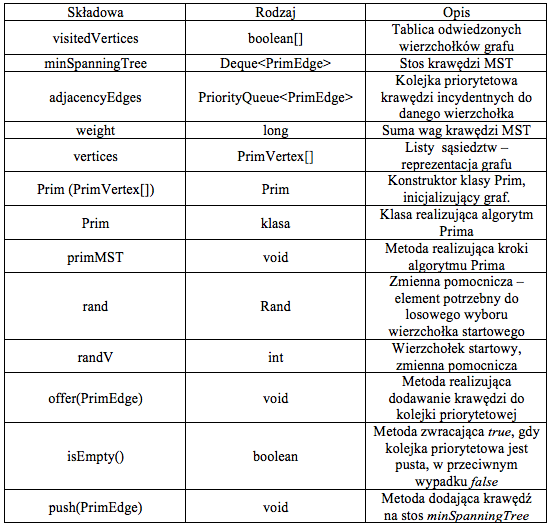
\includegraphics[width=0.7\textwidth]{tex/fig/padd0}
	\caption{Składowe implementacji algorytmu Prima }
	\label{fig: sp}
\end{figure}


Składowe pomocnicze implementacji algorytmu Prima -- rys. \ref{fig: sp}
\begin{figure}[htb!]
	\centering
	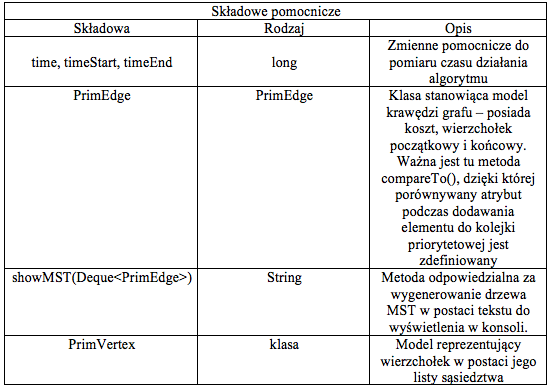
\includegraphics[width=1\textwidth]{tex/fig/padd}
	\caption{Składowe pomocnicze implementacji algorytmu Prima }
	\label{fig: sp2}
\end{figure}

\newpage
Implementacja algorytmu Prima -- rys.\ref{fig: lp1}
\begin{figure}[htb!]
	\centering
	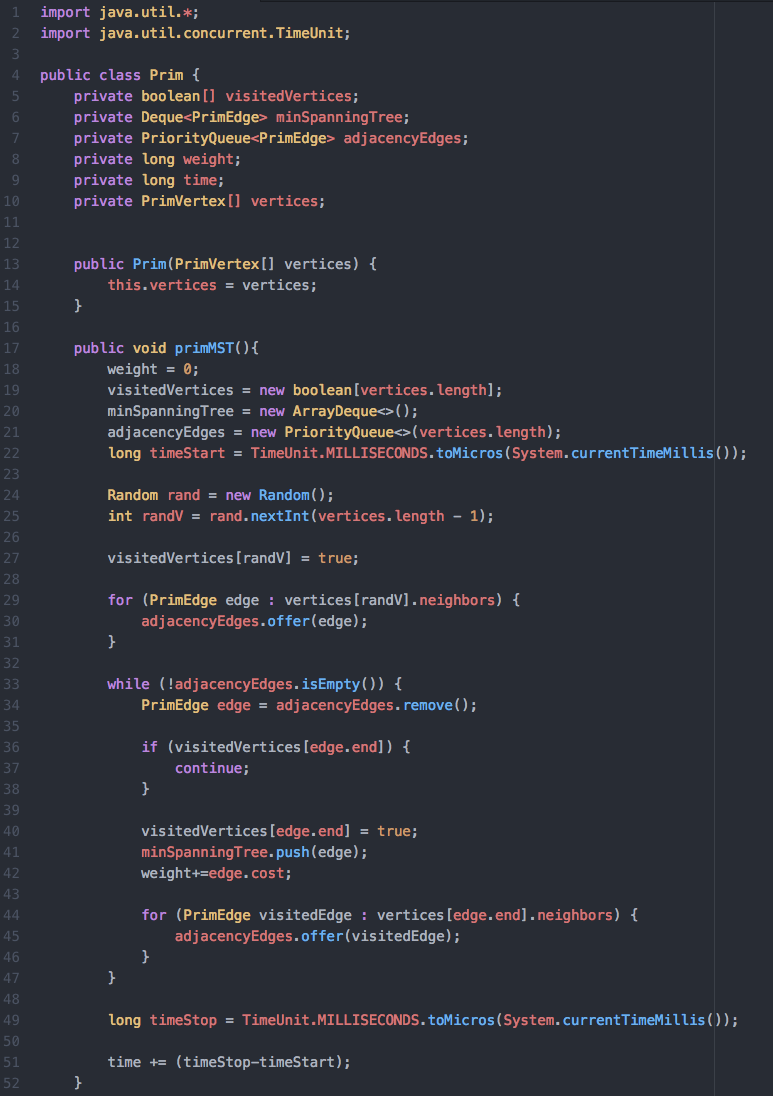
\includegraphics[width=0.9\textwidth]{tex/fig/lp1}
	\caption{Implementacja algorytmu Prima}
	\label{fig: lp1}
\end{figure}

Implementacja algorytmu Prima c.d.-- rys.\ref{fig: lp2}
\begin{figure}[htb!]
	\centering
	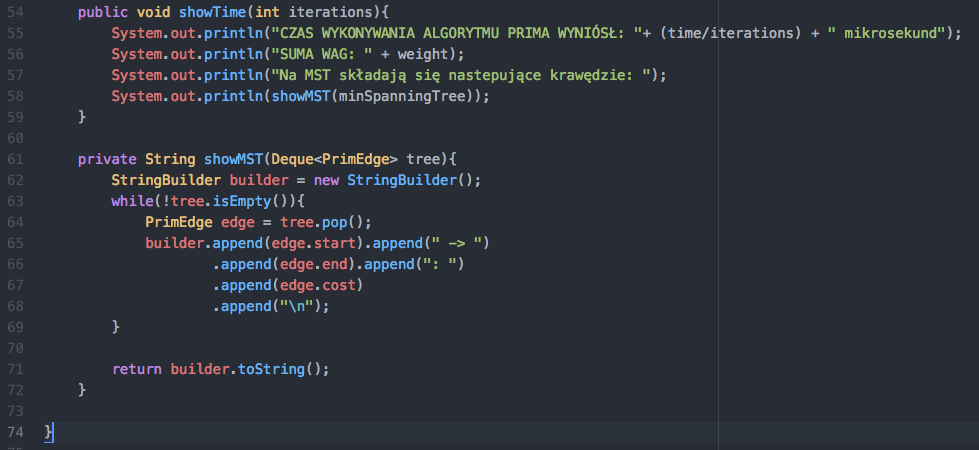
\includegraphics[width=1\textwidth]{tex/fig/lp2}
	\caption{Implementacja algorytmu Prima c.d.}
	\label{fig: lp2}
\end{figure}

Implementacja klas pomocniczych dla algorytmu Prima  -- rys.\ref{fig: lp3}
\begin{figure}[htb!]
	\centering
	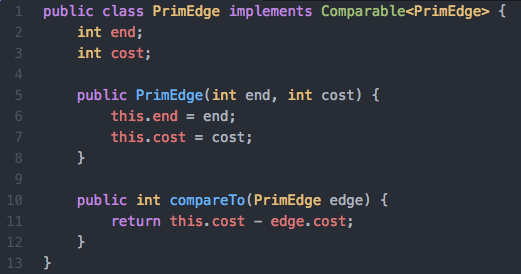
\includegraphics[width=1\textwidth]{tex/fig/lp3}
	\caption{Implementacja klas pomocniczych dla algorytmu Prima}
	\label{fig: lp3}
\end{figure}
\newpage
Implementacja klas pomocniczych dla algorytmu Prima c.d. -- rys.\ref{fig: lp4}
\begin{figure}[htb!]
	\centering
	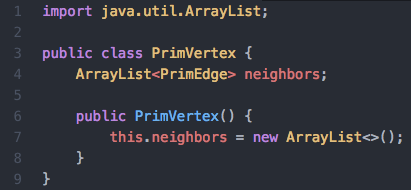
\includegraphics[width=0.6\textwidth]{tex/fig/lp4}
	\caption{Implementacja klas pomocniczych dla algorytmu Prima c.d.}
	\label{fig: lp4}
\end{figure}

\newpage
\section{Kod źródłowy algorytmu Kruskala}
Implementacja struktury zbiorów rozłącznych wykorzystuje techniki kompresji ścieżek oraz scalania po randze. Pozwala to na bardziej efektywne wykonywanie operacji niezbędnych do realizacji algorytmu. Kompresja ścieżek polega na „spłaszczeniu” drzewa, co skraca czas dostępu do poszczególnych elementów. Scalanie po randze natomiast powoduje, że płytsze drzewo jest zawsze dołączane do korzenia głębszego, co pozwala ograniczyć zwiększanie się głębokości drzewa.\\
Składowe implementacji algorytmu Kruskala -- rys. \ref{fig: sk}:\\
\begin{figure}[htb!]
	\centering
	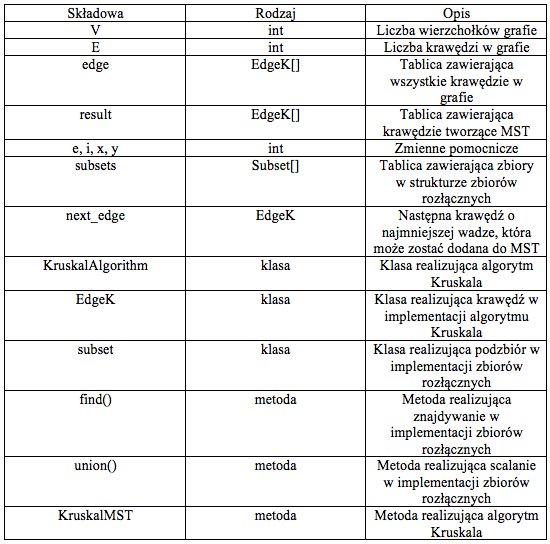
\includegraphics[width=0.8\textwidth]{tex/fig/skladowe_kruskal}
	\caption{Składowe implementacji algorytmu Kruskala}
	\label{fig: sk}
\end{figure}

\newpage
Listing kodu źródłowego implementacji algorytmu Kruskala:\\
\begin{figure}[htb!]
	\centering
	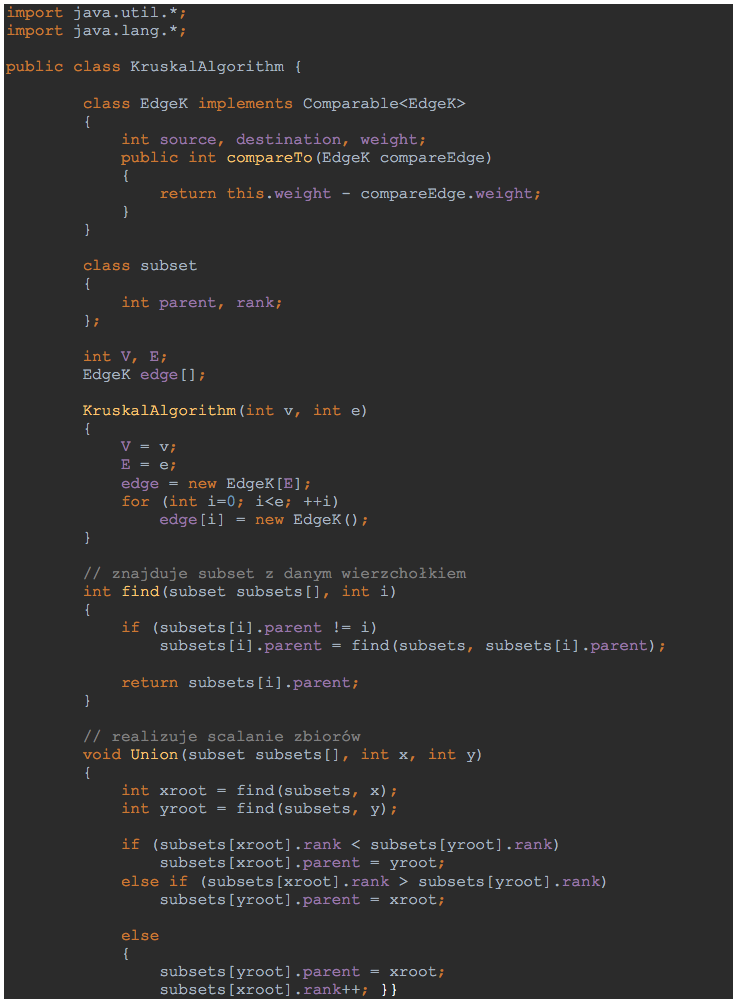
\includegraphics[width=0.9\textwidth]{tex/fig/listing_k1}
	\caption{Implementacja algorytmu Kruskala}
	\label{fig: ik1}
\end{figure}

Listing kodu źródłowego implementacji algorytmu Kruskala c.d.:\\
\begin{figure}[htb!]
	\centering
	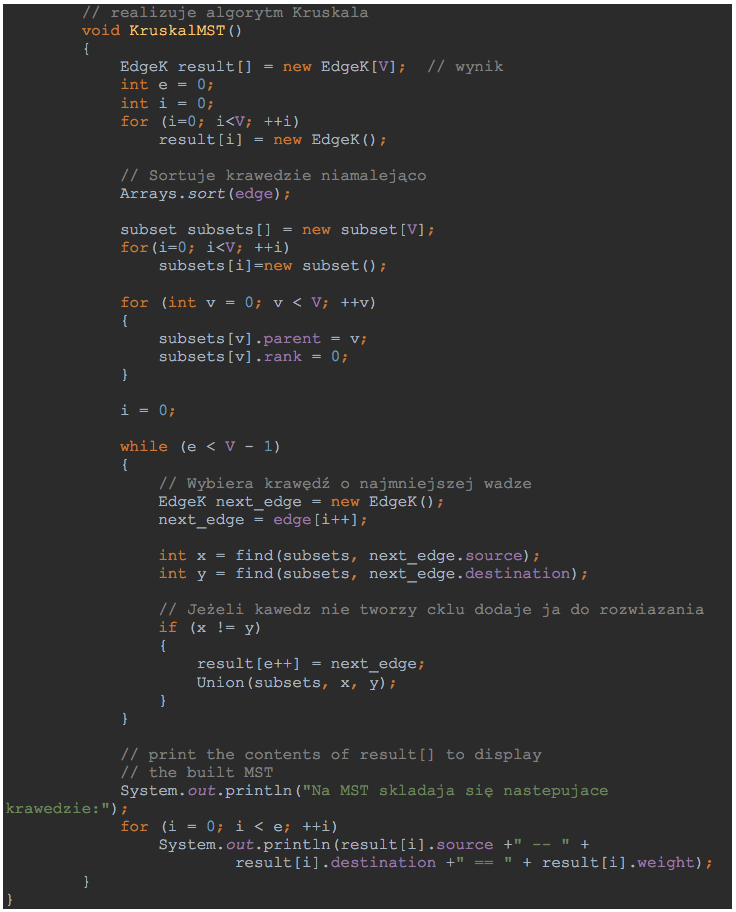
\includegraphics[width=1\textwidth]{tex/fig/listing_k2}
	\caption{Implementacja algorytmu Kruskala c.d.}
	\label{fig: ik2}
\end{figure}
\newpage
\fancyhead[R]{}
\fancyhead[C]{}
\fancyhead[L]{}